\begin{activity} \label{A:3.4.4}  
A trough is being constructed by bending a $4 \times 24$ (measured in feet) rectangular piece of sheet metal.  Two symmetric folds 2 feet apart will be made parallel to the longest side of the rectangle so that the trough has cross-sections in the shape of a trapezoid, as pictured in Figure~\ref{F:3.4.Act4}.  At what angle should the folds be made to produce the trough of maximum volume?
\begin{figure}[h]
\begin{center}
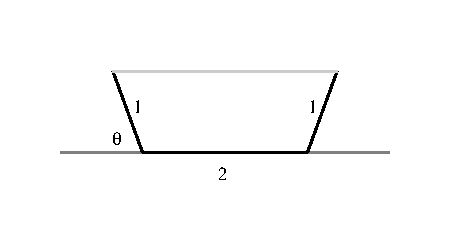
\includegraphics{figures/3_4_Act4.eps}
\caption{A cross-section of the trough formed by folding to an angle of $\theta$.} \label{F:3.4.Act4}
\end{center}
\end{figure}
\end{activity}
\begin{smallhint}
Drop altitudes from the top of the trough to the base of length 2.  In the two triangles that are formed, what are the lengths of the legs in terms of $\theta$?
\end{smallhint}
\begin{bighint}
Drop altitudes from the top of the trough to the base of length 2.  In the two triangles that are formed, what are the lengths of the legs in terms of $\theta$?  What is the overall area in terms of $\theta$?  (Note that since the length of the trough is constant, the volume will be maximized by maximizing cross-sectional area.)  Finally, after you differentiate $A(\theta)$, use the identity $\sin^2(\theta) = 1 - \cos^2(\theta)$ to write $A'(\theta)$ solely in terms of the cosine function and note that the result is a quadratic equation in $\cos(theta)$.
\end{bighint}
\begin{activitySolution}
Once we choose the angle $\theta$, the two right triangles in the trapezoid are determined, and each has a horizontal leg of length $\cos(\theta)$ and a vertical leg of length $\sin(\theta)$.  Thus, the sum of the areas of the two triangles is $\sin(\theta) \cos(\theta)$, and the area of the rectangle between them is $2\sin(theta)$.  Hence, the area of the trapezoidal cross-section is $A(\theta) = \sin(\theta) \cos(\theta) + 2 \sin(\theta)$.  Because the length of the trough is constant, the trough's volume will be maximized by maximizing cross-sectional area.  Note, too, that the domain for $\theta$ is $0 \le \theta \le \frac{\pi}{2}$.

Differentiating, we find that
$$A'(\theta) = \sin(\theta) (-\sin(\theta)) + \cos(\theta) \cos(\theta) + 2 \cos(\theta) = -\sin^2(\theta) + \cos^2(\theta) + 2 \cos(\theta).$$
Using the identity $\sin^2(\theta) = 1 - \cos^2(\theta)$, it follows that
$$A'(\theta) = \cos^2(\theta) - 1 + \cos^2(\theta) + 2 \cos(\theta) = 2\cos^2(\theta) + 2 \cos(\theta) - 1.$$
This most recent equation is quadratic in $\cos(\theta)$, so letting $u = \cos(\theta)$, we can start to solve the equation $A'(\theta) = 0$ by solving $2u^2 + 2u - 1 = 0$.  Doing so, we find that 
$$u = \frac{-1 \pm \sqrt{3}}{2} \approx 0.3660254, -1.3660254,$$
so only $u = \frac{-1 + \sqrt{3}}{2}$ will be a potential value of the cosine function from an angle that lies in the interval $[0,\frac{\pi}{2}]$.  Now, recalling that $\cos(\theta) = u$, to find the critical value $\theta$, we solve $\cos(\theta) = \frac{-1 + \sqrt{3}}{2}$, which implies $\theta = \arccos(\frac{-1 + \sqrt{3}}{2}) \approx 1.19606$ radians, or $\theta \approx 68.5292^\circ$.

Finally, to confirm that $A$ has an absolute maximum at $\theta = \arccos(\frac{-1 + \sqrt{3}}{2}) \approx 1.19606$, we consider this value as well as the endpoints of $[0, \frac{\pi}{2}]$, and evaluate $A$ to find that $A(0) = 0$, $A(\frac{\pi}{2}) = 2$, and $A(1.19606) \approx 2.2018$, which is the absolute maximum possible cross-sectional area.
\end{activitySolution}
\aftera